\documentclass[a4paper,10pt,twocolumn]{ltjsarticle}
\usepackage[haranoaji]{luatexja-preset}
\usepackage[top=18mm,bottom=20mm,left=17mm,right=17mm,columnsep=8mm]{geometry}
\usepackage{graphicx,booktabs,array,caption,enumitem,xcolor,tikz}
\usetikzlibrary{shapes.geometric}
\setlength{\parindent}{1\zw}
\renewcommand{\baselinestretch}{1.0}
\setlength{\parskip}{0pt}
\renewcommand{\thesection}{\arabic{section}.}
\renewcommand{\thesubsection}{\arabic{section}.\arabic{subsection}.}
\makeatletter
\renewcommand{\section}{\@startsection{section}{1}{\z@}{1.1\Cvs \@plus.4\Cdp \@minus.2\Cdp}{.5\Cvs \@plus.2\Cdp}{\normalfont\gtfamily\bfseries\large}}
\renewcommand{\subsection}{\@startsection{subsection}{2}{\z@}{.8\Cvs \@plus.3\Cdp \@minus.2\Cdp}{.3\Cvs \@plus.1\Cdp}{\normalfont\gtfamily\bfseries\normalsize}}
\makeatother
\captionsetup{font={small,sf},labelsep=space,justification=raggedright,singlelinecheck=false,skip=3pt}
\captionsetup[table]{position=top}
\setlist[itemize]{leftmargin=1.2\zw,itemsep=0pt,topsep=2pt,parsep=0pt}
\setlength{\textfloatsep}{8pt plus 2pt minus 2pt}
\setlength{\floatsep}{8pt plus 2pt minus 2pt}
\setlength{\intextsep}{8pt plus 2pt minus 2pt}
\pagestyle{plain}
\raggedbottom
\begin{document}
\twocolumn[{
\noindent\fbox{\gtfamily\small\ 生成AI論文\ }\par\medskip
\begin{center}
{\gtfamily\bfseries\LARGE 理系の学科に女性はどれだけ入学しているのか：学校基本調査の58の学科区分で比べる$^{\dagger}$}\par\medskip
{\gtfamily\bfseries\large 大学（学部）入学者の女性比率の学科差と入学者数との関連（令和5〜7年度）}\par\medskip
{\normalsize EduData調査研究グループ$^{*1}$・教育データサイエンス解析班$^{*2}$}\par
{\small オープン教育統計推進プロジェクト$^{*1}$・初等中等STEM教育データ基盤ユニット$^{*2}$}
\end{center}\smallskip
\noindent\begin{minipage}{\textwidth}\small 本研究は，学校基本調査（令和5〜7年度）の公表値から，大学（学部）の関係学科58区分の入学者の女性比率を整理した．令和7年度の全体は47.0\%で，区分ごとには8.2\%から94.2\%まで分かれた．最も低いのは工学・機械工学（8.2\%）で，電気通信工学（12.2\%），理学・物理学（15.6\%）が続いた．重みづけた比率は工学20.4\%，理学32.1\%であった．理学の生物学（2726人）は47.1\%，工学で最も高い工芸学（49.5\%）は564人の小さな区分で，除くと工学の最大は応用化学の34.1\%であった．志願者の女性比率と入学者数に大きな関連は見られなかった（\textit{r}=-.03，\textit{BF}\textsubscript{10}=0.11）．これらは集計値であり，進路選択の理由や入試の公平さは示さない．\par\smallskip
\noindent{\gtfamily キーワード：}学校基本調査，大学入学者，女性比率，理工系，生態学的誤謬\end{minipage}\medskip
}]
\let\thefootnote\relax
\footnotetext{\footnotesize 2026年10月執筆\\ $^{\dagger}$How Many Women Enter Science and Engineering Departments? A Comparison of 58 Department Categories in the Japanese School Basic Survey\\ $^{*1}$ Open Education Data Project, Tokyo, Japan\quad $^{*2}$ Educational Data Science Unit, Tokyo, Japan}
\section{はじめに}
\subsection{研究の背景}
理学・工学に進む女性が少ないことは，長く論じられてきた．Blickenstaff (2005)は，これを段階ごとに人が抜ける「漏れるパイプライン」と見るか，性別によるふるい分けと見るかという問いとして整理した．数学の男女差については，Else-Quest et al. (2010)が国ごとのパターンをメタ分析し，Guiso et al. (2008)は文化との関係を論じ，Spencer et al. (1999)はステレオタイプ脅威を検討した．Su et al. (2009)は興味の性差をメタ分析し，Lent et al. (1994)は興味・選択・遂行を社会的認知の枠組みで捉える理論を示した．Cheryan et al. (2017)はSTEMの中でも男女の構成が分野によって異なる理由を問うており，「理系」を学科の単位で比べることには意味がある．

日本では経済産業省 (2019)がIT人材の需給を調査するなど，理工系・情報系の人材への関心が高い．学校基本調査の「関係学科別 大学入学状況」（文部科学省，2025）は，全国の大学（学部）の入学者と志願者を関係学科の小分類ごとに男女別に示す．ただし「情報」の独立した区分はない．また女性比率は入学した（志願した）人の男女比であり，進路を選んだ理由や入試の公平さは示さない．
\subsection{リサーチクエスチョン}
本研究の目的は，学校基本調査の公表値から，大学（学部）入学者の女性比率の学科による違いを記述し，理学・工学の各学科の位置を確かめることである．

志願者との違いと3年度間の変化を補足する．
\begin{itemize}
\item RQ1：関係学科別に入学者の女性比率はどう違い，理学・工学の各学科はどこに位置するか（令和7年度）．
\item RQ2：入学者数の多い学科ほど，入学者の女性比率は高いか低いか（58区分の関連として）．
\end{itemize}
\section{調査対象および分析方法}
e-Statに掲載された学校基本調査（毎年5月1日現在）の統計表「関係学科別 大学入学状況」の令和5〜7年度のExcelから，関係学科の小分類ごとに入学者と入学志願者の男女別の値を機械的に取り込み，女性の人数を男女計で割って女性比率（\%）を求めた．小分類の合計が大分類の計と一致することを確かめた．対象は大学（学部）で，短期大学と大学院は含まない．3年度すべてで入学者が200人以上の58区分を用いた．令和7年度の入学者全体は645,513人（女性303,073人）である．大分類の比率は入学者数で重みづけた．

RQ2では，入学者の女性比率が入学者数を分母とするため，計算上のつながりを避けて入学志願者の女性比率を代わりに用いた（両者は\textit{r}=.99でほぼ同順）．相関は\textit{r}，95\%信頼区間，スピアマンの\textit{ρ}，\textit{p}，JZSベイズファクター\textit{BF}\textsubscript{10}で示し，\textit{BF}\textsubscript{10}が3を超えれば関連を支持，1/3未満なら関連がないことを支持とみなした．4指標の全ペアを探索し，計算でつながる組を除いて研究課題に関わる組だけを報告した．多重比較による偶然の関連が含まれうる．各区分は同じ重みで扱った．
\begin{table*}[!t]
\caption{主要指標の基本記述統計量}
\centering\small
\begin{tabular}{>{\raggedright\arraybackslash}p{9.2cm}rrrrrr}
\toprule
指標 & \textit{K} & 平均 & \textit{SD} & 中央値 & 最小 & 最大 \\
\midrule
入学者数 & 174 & 10948.4 & 17380.9 & 4265.5 & 200.0 & 118344.0 \\
女性の入学者数 & 174 & 5095.3 & 7297.7 & 2409.0 & 21.0 & 38685.0 \\
入学者の女性比率（\%） & 174 & 47.0 & 21.9 & 44.3 & 7.1 & 94.3 \\
入学志願者の女性比率（\%） & 174 & 45.4 & 21.3 & 42.4 & 8.0 & 95.9 \\
\bottomrule
\end{tabular}
\par\smallskip{\footnotesize 注）単位は人，\textit{K}は観測数（国・地域）．}
\end{table*}
\begin{table*}[!t]
\caption{主要指標間のピアソンの相関係数と，ベイズファクター}
\centering\small
\begin{tabular}{>{\raggedright\arraybackslash}p{6.4cm}>{\raggedright\arraybackslash}p{6.4cm}rrr}
\toprule
指標 \textit{X} & 指標 \textit{Y} & \textit{r} & \textit{p} & \textit{BF}\textsubscript{10} \\
\midrule
入学者数 & 入学者の女性比率（\%） & -.01 & = .874 & 0.06 \\
入学者数 & 入学志願者の女性比率（\%） & -.02 & = .762 & 0.06 \\
入学者の女性比率（\%） & 入学志願者の女性比率（\%） & .99 & < .001 & >1000 \\
\bottomrule
\end{tabular}
\par\smallskip{\footnotesize 注）\textit{BF}\textsubscript{10}はJZSベイズファクター（3を超えれば関連を支持，1/3を下回れば関連がないことを支持）．全ペアの探索の一部を載せた．}
\end{table*}
\section{結果}
RQ1について，令和7年度の58区分の女性比率は平均47.61\%，中央値46.55\%，標準偏差21.66で，最小8.2\%，最大94.2\%であった．20\%未満は7区分，70\%を超えるのは7区分であった．最も高いのは家政・児童学（94.2\%），家政・家政学（93.4\%），保健・看護学（91.3\%）であった．最も低いのは工学・機械工学（8.2\%）で，工学・電気通信工学（12.2\%），理学・物理学（15.6\%），工学・応用理学（15.8\%）が続いた．人数では，機械工学は入学者12719人のうち女性1041人，電気通信工学は24684人のうち3007人，物理学は2418人のうち378人，数学は3682人のうち775人（21.0\%）であった．数学の比率は中央値の半分に満たなかった．

入学者数で重みづけた大分類の比率は，家政88.4\%，芸術69.8\%，保健67.9\%，人文科学63.8\%，教育57.0\%，農学48.5\%，社会科学38.7\%，理学32.1\%，工学20.4\%であった．大分類の中の幅は大きく，工学の9区分は8.2\%から49.5\%，理学の6区分は15.6\%から47.1\%であった．ただし工学の最大の49.5\%は入学者564人の工芸学で，これを除くと最大は応用化学の34.1\%である．理学の最大は入学者2726人の生物学であった．

志願者の女性比率も入学者とほぼ同じ並びで，最も低いのは工学・機械工学（9.5\%），工学・電気通信工学（13.2\%）であった．入学者の比率から志願者の比率を引いた差は平均1.56ポイントで，入学者のほうが高い区分が41，低い区分が17，差が1ポイント以内の区分は15（上の41と17の内数）であった．この差は男女比の違いを示すだけで，入試の公平さを示すものではない．

RQ2について，入学者数は中央値4308.5人，平均11117.02人と偏っており，最大は商学・経済学の118344人，最小は商船学の204人であった．入学者数と志願者の女性比率の相関は\textit{r}=-.03（95\%CI [-.29, .23]，\textit{ρ}=.10，\textit{n}=58，\textit{p}=.804，\textit{BF}\textsubscript{10}=0.11）で，大きな関連は見られず，\textit{BF}\textsubscript{10}は関連がないことを支持する範囲にあった．ただし信頼区間は.23まで含み，\textit{r}と\textit{ρ}で符号が異なる．入学者の女性比率を直接用いても\textit{r}=-.02であった（分母を共有するため参考値）．入学者の多い社会科学（209454人）は38.7\%，人文科学（87837人）は63.8\%であった．

補足として，令和5年度から7年度にかけて，女性比率は39区分で上がり，18区分で下がった（平均0.98ポイント）．上がり幅が大きいのは工学・工芸学（564人，6.7ポイント），理学・生物学（5.7ポイント），工学・応用化学（5.1ポイント）であった．入学者の少ない区分は比率が揺れやすく，時点も3つだけである．
\begin{figure}[t]\centering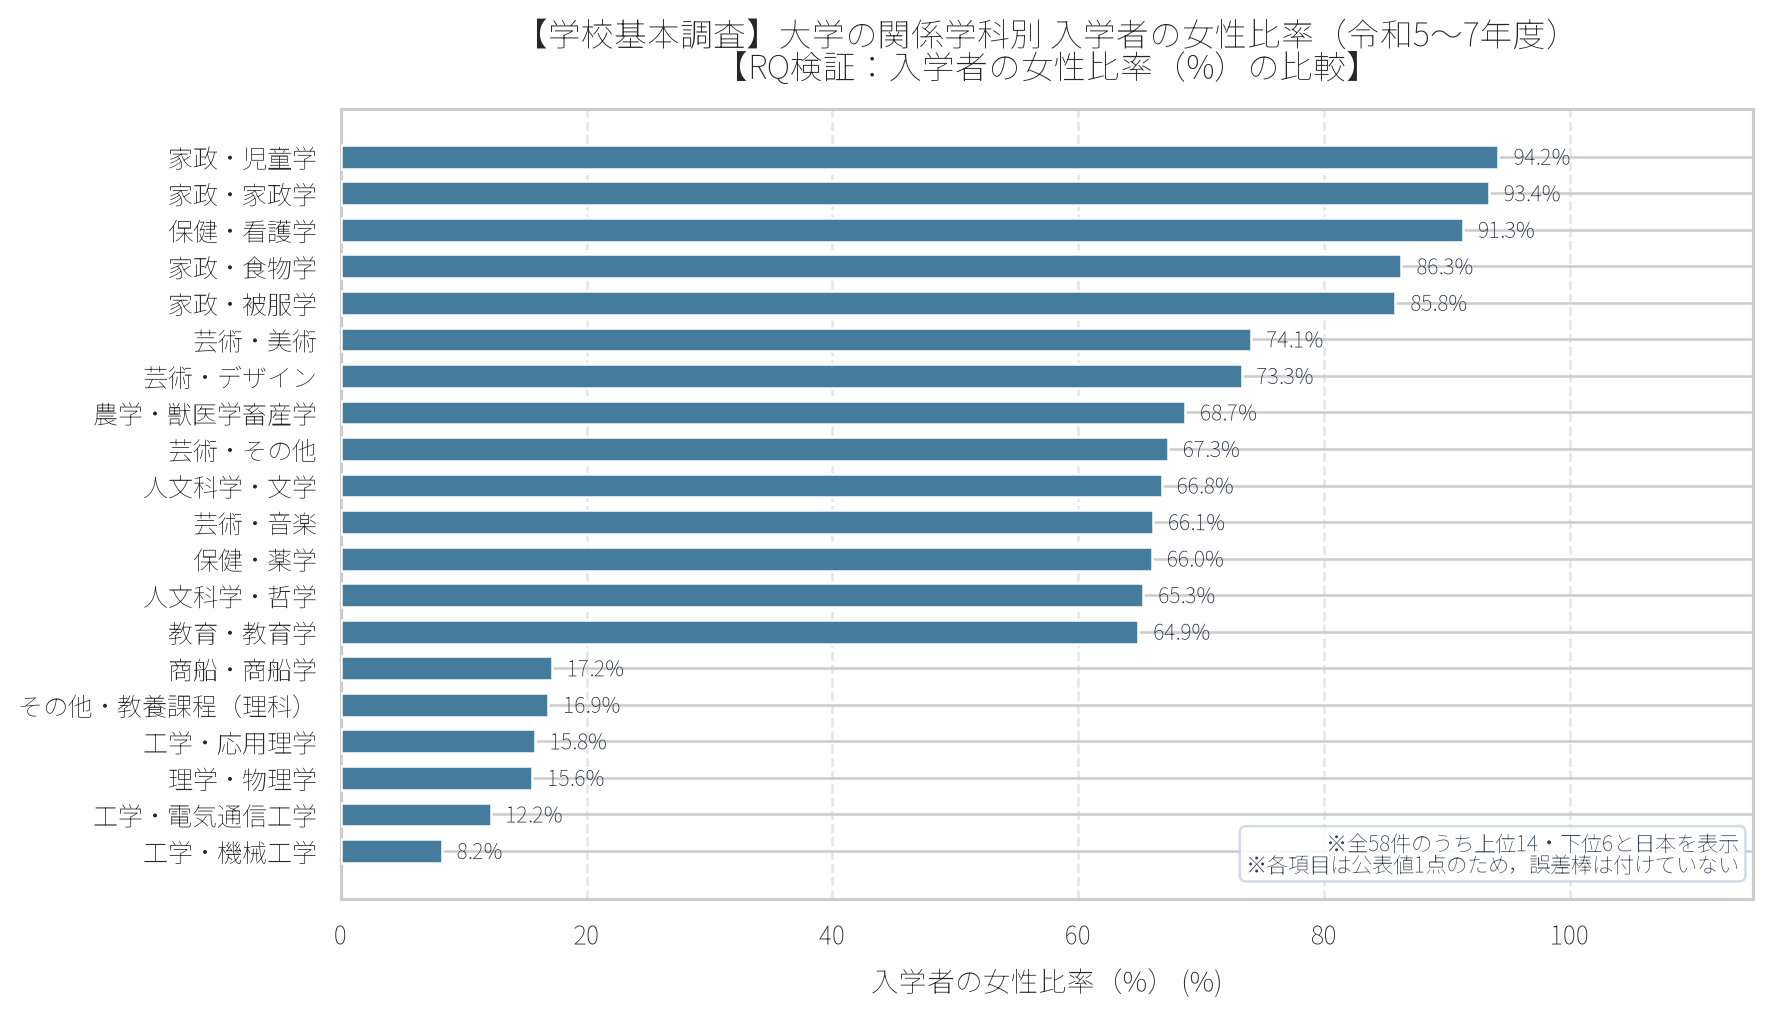
\includegraphics[width=\columnwidth]{chart_japan_stem_cs_enrollment.png}\caption{入学者の女性比率（\%）の値の比較（上位・下位と日本を抜粋）}\end{figure}
\begin{figure}[t]\centering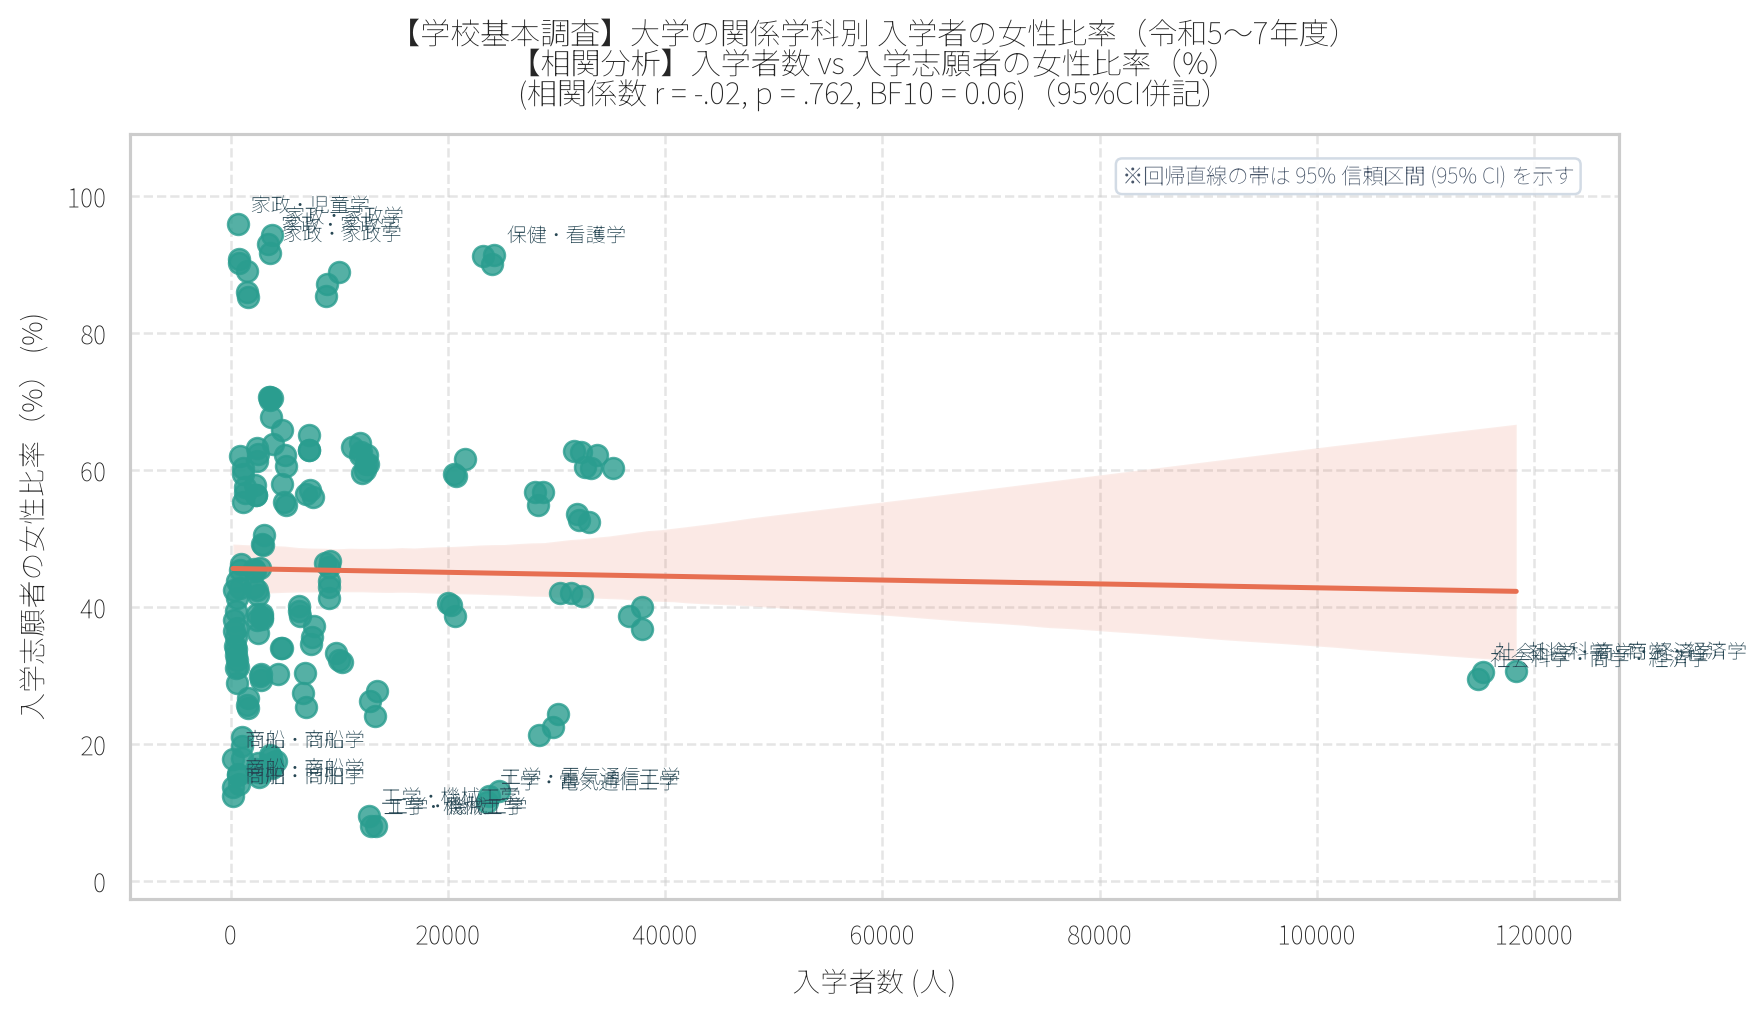
\includegraphics[width=\columnwidth]{chart_secondary_japan_stem_cs_enrollment.png}\caption{入学者数と入学者の女性比率（\%）の関連（回帰直線と95\%信頼区間の帯）}\end{figure}
\section{考察}
RQ1の結果，入学者の女性比率は全体で47.0\%である一方，区分によって8.2\%から94.2\%まで異なった．20\%未満の7区分のうち5区分は理学・工学で，残りは理科の教養課程と商船であった．ただし応用化学（34.1\%），土木建築工学（29.5\%），理学の生物学（47.1\%）のように中位にある大きな区分もある．工芸学（49.5\%）は564人の小さな区分であり，これだけで「工学にも高い区分がある」とは言えない．Cheryan et al. (2017)が問うたように，「理系」をひとまとめにすると分野の違いは見えなくなるが，同論文の議論が日本の学科差にどこまで当てはまるかは確かめられない．

RQ2では大きな関連は見られなかったが，信頼区間には幅があり，関連が全くないとは言えない．また，204人の区分と118344人の区分を同じ重みで扱っている．

女性比率が低い理由は，本研究のデータでは検証できない．Su et al. (2009)の興味の性差の知見と，機械工学や電気通信工学で低く看護学や児童学で高いという並びは矛盾しないが，集計値から個人の興味を読み取ることはできない（生態学的誤謬）．なお電気通信工学に情報系の学科が含まれるかは確認していない．Else-Quest et al. (2010)，Guiso et al. (2008)，Spencer et al. (1999)は成績や態度を扱った研究であり，進路への影響は別の問題である．ステレオタイプ脅威には効果の大きさをめぐる議論もある．Lent et al. (1994)の理論が示すように進路の選択は興味や遂行と結びつくが，入学者の表が示すのは選択の結果だけであり，これらの要因の寄与は仮説にとどまる．

Blickenstaff (2005)の問いに照らすと，本研究が見たのは大学入学という一つの段階にすぎない．機械工学（志願者9.5\%，入学者8.2\%）や物理学（志願者16.0\%，入学者15.6\%）では，志願の段階ですでに女性比率が低い．ただし志願者が延べで数えられているかは確かめておらず，入試の公平さについては何も言えない．経済産業省 (2019)が示すように情報系の人材への関心は高いが，この表には「情報」の区分がない．

教育現場では，「理系」の中でも学科によって女性比率が大きく違うという事実を進路学習で示すことが考えられるが，その効果は確かめられていない．

本研究の限界は，(1)集計値のみで個人の理由や因果を特定できないこと，(2)成績・興味・家庭などの交絡を統制していないこと，(3)悉皆の集計で標本抽出の誤差はないが，区分は表の分類に依存し，200人未満の小分類と「情報」を扱えないこと，(4)主に1時点の横断比較で，変化も3時点に限られ，小さい区分は比率が揺れやすいこと，(5)RQ2で代わりの指標を用いたこと，である．
\section*{参考文献}
\begingroup\scriptsize\setlength{\parindent}{0pt}\raggedright
\par\hangindent=1.5\zw\hangafter=1 BLICKENSTAFF, J. C. (2005) Women and science careers: Leaky pipeline or gender filter? Gender and Education, \textbf{17} (4) ：369-386.\vspace{1pt}
\par\hangindent=1.5\zw\hangafter=1 CHERYAN, S., ZIEGLER, S. A., MONTOYA, A. K. and JIANG, L. (2017) Why are some STEM fields more gender balanced than others? Psychological Bulletin, \textbf{143} (1) ：1-35.\vspace{1pt}
\par\hangindent=1.5\zw\hangafter=1 ELSE-QUEST, N. M., HYDE, J. S. and LINN, M. C. (2010) Cross-national patterns of gender differences in mathematics: A meta-analysis. Psychological Bulletin, \textbf{136} (1) ：103-127.\vspace{1pt}
\par\hangindent=1.5\zw\hangafter=1 GUISO, L., MONTE, F., SAPIENZA, P. and ZINGALES, L. (2008) Culture, gender, and math. Science, \textbf{320} (5880) ：1164-1165.\vspace{1pt}
\par\hangindent=1.5\zw\hangafter=1 経済産業省 (2019) IT人材需給に関する調査 調査報告書. 経済産業省.\vspace{1pt}
\par\hangindent=1.5\zw\hangafter=1 LENT, R. W., BROWN, S. D. and HACKETT, G. (1994) Toward a unifying social cognitive theory of career and academic interest, choice, and performance. Journal of Vocational Behavior, \textbf{45} (1) ：79-122.\vspace{1pt}
\par\hangindent=1.5\zw\hangafter=1 文部科学省 (2025) 学校基本調査 令和7年度 統計表『関係学科別 大学入学状況』. 政府統計の総合窓口（e-Stat）.\vspace{1pt}
\par\hangindent=1.5\zw\hangafter=1 SPENCER, S. J., STEELE, C. M. and QUINN, D. M. (1999) Stereotype threat and women's math performance. Journal of Experimental Social Psychology, \textbf{35} (1) ：4-28.\vspace{1pt}
\par\hangindent=1.5\zw\hangafter=1 SU, R., ROUNDS, J. and ARMSTRONG, P. I. (2009) Men and things, women and people: A meta-analysis of sex differences in interests. Psychological Bulletin, \textbf{135} (6) ：859-884.\vspace{1pt}
\endgroup
\section*{Summary}
{\footnotesize\setlength{\parindent}{0pt}Using published values from the School Basic Survey by the Ministry of Education, Culture, Sports, Science and Technology for 2023 to 2025, we described the share of women among new undergraduate entrants in 58 department categories. In 2025 the overall share was 47.0\%, but it ranged from 8.2\% to 94.2\% across categories. The lowest shares were in mechanical engineering (8.2\%), electrical and communication engineering (12.2\%) and physics (15.6\%); mathematics was 21.0\%. Weighted by the number of entrants, the share was 20.4\% in engineering and 32.1\% in science, compared with 88.4\% in home economics and 67.9\% in health. The highest share in engineering (49.5\%) was a small category of 564 entrants; excluding it, the maximum in engineering was 34.1\%, while biology in science (2,726 entrants) reached 47.1\%. To avoid a computational link with the denominator, we used the share of women among applicants; it showed no large association with the number of entrants (r = -.03, BF10 = 0.11). These are associations between aggregate values for department categories and do not show the reasons for students' choices or the fairness of admissions.\par\smallskip KEYWORDS: SCHOOL BASIC SURVEY, UNIVERSITY ENTRANTS, WOMEN IN STEM, DEPARTMENT COMPARISON, ECOLOGICAL FALLACY\par}
\medskip\noindent\fbox{\parbox{\dimexpr\columnwidth-2\fboxsep-2\fboxrule}{\footnotesize\gtfamily 【付記：生成AIによる自動執筆に関する開示】\\ 本論文は学生への教育目的で作成している．使用しているデータは公的オープンデータである．統計の算出はPythonで行い，文章は生成AI（Anthropic Claude等）を活用して作成した．記載した統計数値は元データに準拠しているが，教育学的な考察や提言の妥当性は，指導現場の実情に応じて，批判的に吟味してほしい．}}
\end{document}
